\chapter{Columnar Storage}
\label{c:columnar-storage}

In this chapter, we explore the application of columnar data structures for different storage components of the \gls{gdbms}, to meet the desiderata we outlined in Chapter~\ref{c:guidelines}. Section \ref{sec:vertex-property-columns} describes the design of columns to store vertex properties and a new compact vertex identification scheme that accompanies the design. In Section \ref{sec:edge-property-columns}, we start by describing the two columnar storage designs to store edge properties and their pros and cons. Then, we propose a third design, \textcolor{red}{paged edge property list}, that is a sweet spot between the earlier two designs and the one we adopt as an optimum design for storing edge properties. Similar to Section~\ref{sec:vertex-property-columns}, we describe a novel and compact edge identification scheme that accompanies our design from edge property columns. \textcolor{red}{As we observed earlier, adjacency lists are already columnar structures.} Section~\ref{sec:adjacency-lists} describes several storage optimizations to the adjacency lists to reduce the system's memory footprint without sacrificing query performance, using the type of structures we observed in guideline~\ref{gdln:graph-schema}.

\section{Columns for Vertex Properties}
\label{sec:vertex-property-columns}

\begin{figure}
	\vspace{-25pt}
	\hfill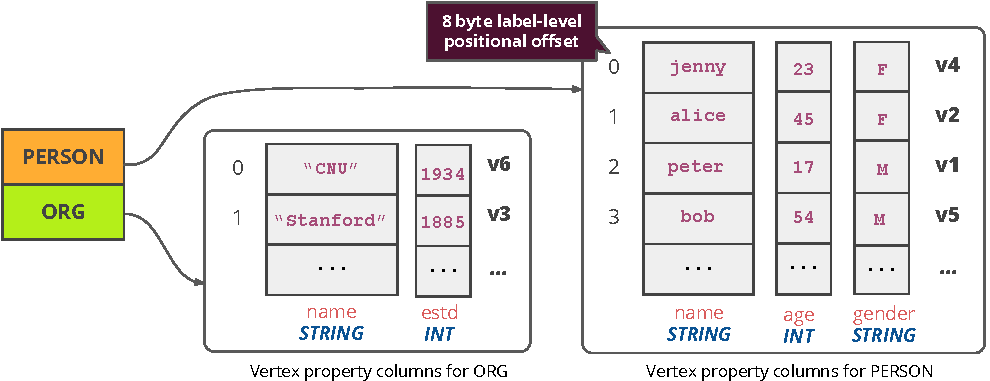
\includegraphics[scale=0.85]{img/vpcols}\hspace*{\fill}
	\caption{Vertex property columns for the graph in Figure~\ref{fig:runn}.}
	\label{fig:vpcols}
	\vspace{-8pt}
\end{figure}

Columnar data-structures can be directly used for storing vertex properties. Let $(lv_1, lv_2, ...)$ be the vertex labels in a graph. Let $p_{i,1},  p_{i,2}, ... p_{i, n}$ be the structured vertex properties of $lv_i$, with a datatype $d_{i,j}$. We define a \emph{vertex property column} for each $p_{i,j}$, having a fixed data type $d_{i,j}$. Each column stores the value of a single property $p_{i,j}$ for all vertices having $lv_i$ at consecutive locations. We call the collection of columns of all properties of a particular vertex label $lv_i$, the \emph{vertex property column family} of $lv_i$. All property values of a particular vertex $v$, with label $lv_i$, is located at the same positional offset in their respective columns in column family of  $lv_i$. We call this positional offset, \emph{(vertex) label-level positional offset} of vertex $v$.

% reading a property.

Ideally, the property value of a vertex should directly be read using the ID of the vertex as the positional offset in the column. However, \gls{gdbms} typically gives globally unique 8-byte consecutive IDs to all the vertices in the system, irrespective of their labels. That means ID 0 can be given to a vertex with label PRESION and 1 to the vertex with label ORG. We cannot use this ID scheme as the positional offset for the above design. One possible solution is to maintain a map for each label, from the vertex's \enquote{global} ID to its \enquote{local}, i.e, a label-level positional offset of a vertex in the column. This, however, requires extra storage for maintaining the map and one level of indirection when accessing the vertex properties. Instead, we identify a vertex by a \emph{\textbf{(vertex label, label-level positional offset)}} tuple in the system in place of global vertex ID. This allows direct access to the properties by using the positional offset which now is part of the vertex ID. However, using this new vertex ID scheme requires materializing 2 pieces of information in the adjacency lists - a vertex label and a local positional offset, compared to only global vertex ID by the earlier scheme. This increases the memory overhead as the \enquote{local} positional offsets and the global vertex ID are of the same size. However, as we will show in section \ref{sec:storage-optimizations}, we can often avoid storing the vertex labels with vertex IDs and even save space by using fewer bytes for local positional offsets than the bytes needed by the global vertex IDs.

For reference, figure~\ref{fig:vpcols} shows set of vertex property columns for our example graph in figure~\ref{fig:runn}. It has 2 column families, one for each vertex label, with a column for each structured property of the label. The global vertex IDs on the right of a column family indicates the positional offset at which the properties of a particular vertex are located in the columns of a family. For instance, the properties of vertex $v2$ appear at offset $1$ in columns of PERSON's family. By the new vertex ID scheme, $v2$ is identified as \texttt{PRESON:1}. 

% updates.

The design of the vertex property columns allows for easy insertions and deletions of the vertex properties. Since we cannot localize vertex reads by ordering the properties (Guideline~\ref{gdln:vertices-unordered}), the vertex property columns are unordered. This makes insertions easy which are done by either appending the vertex properties to the appropriate column family and assigning a new vertex ID, or reusing the ID of a previously deleted vertex with the same label. Deleting a property from a column is simply overwriting the property value by a \texttt{NULL} symbol while deleting a vertex involves removing all the edges to/from that vertex from adjacency lists and the ID is recycled. 

\section{Columns for Edge properties}
\label{sec:edge-property-columns}

Recall from Guideline~\ref{ssec:edges-ordered} that edges and edge properties  are read by the \texttt{JOIN} operators in the order they appear in the adjacency lists. We know that the \gls{gdbms} already stores the edges, i.e the edge ID and the neighbour vertex ID, consecutively in the adjacecy lists. Ideally, edge properties should also be stored in the same order. However, as we discuss in this section, this is not possible without replication. We begin by presesnting two columns storage designs for storing edge properties which can be seen as opposite ends of a design spectrum, optimizing the system for \emph{storage} and \emph{performance} respectively:

\begin{figure}
	\vspace{-30pt}
	\hspace*{-20pt}
	\begin{subfigure}{0.45\textwidth}
		\vspace{20pt}
		\centering
		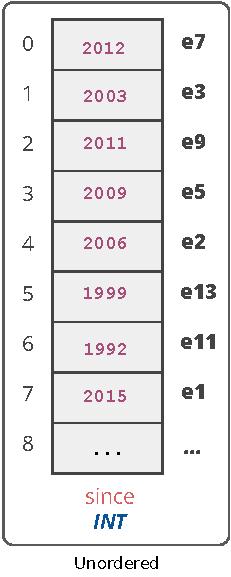
\includegraphics[scale=0.75]{img/sol1}
		\captionsetup{justification=centering}
		\vspace{10pt}
		\caption{Sol 1: (Unordered, No Replication)}
		\label{fig:sol1}
	\end{subfigure}
	\begin{subfigure}{0.55\textwidth}
		\centering
		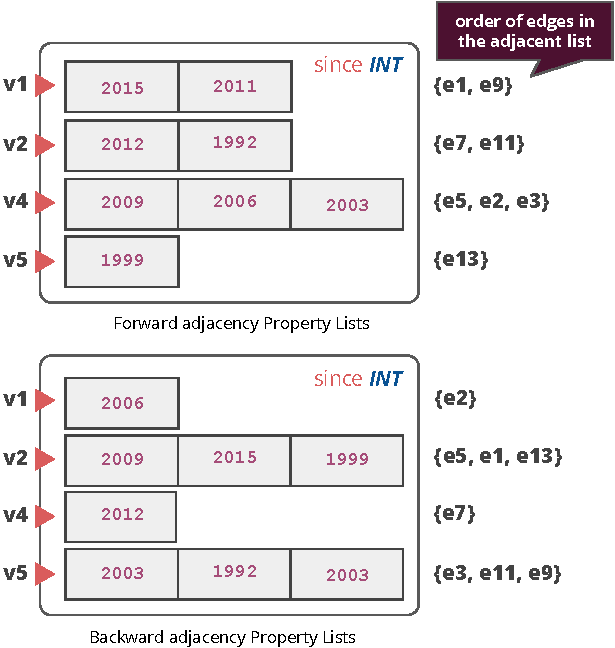
\includegraphics[scale=0.75]{img/sol2}
		\captionsetup{justification=centering}
		\caption{Sol 2: (Ordered, Replication)}
		\label{fig:sol2}
	\end{subfigure}
	\captionsetup{justification=centering}
	\vspace{5pt}
	\caption{Edge property columns in Solution 1 and 2 for \texttt{since} property in Figure~\ref{fig:runn}.}
	\vspace{-10pt}
	\label{fig:sol1and2}
\end{figure}

\vspace{-12pt}
\subparagraph{Solution 1: (Unordered, No replication)}One possibility is to use the columnar storage design similar to that for storing the vertex properties. That is, we have one edge property column for each $q_{i,j}$, where $q_{i,j}$ is a structured property of edge label $l_i$. Edges in the system with this solution can be identified as \emph{(edge label, label-level positional offset)}. However, such a design would not localize the properties of the edge according to their appearance in the adjacency lists, so cannot provide sequential reads when reading the edge properties. Figure~\ref{fig:sol1} shows how this particular design would look like. The figure shows a column with property values for property \texttt{since} for FOLLOWS edges. The property values are not ordered. For our example, the forward adjacency list of \texttt{v4} contains edges \texttt{e5}, \texttt{e2} and \texttt{e3}, whose \texttt{since} property values (at positional offsets 3, 4 and 1) are not stored together in the edge property column. 

\vspace{-12pt}

\subparagraph{Solution 2: (Ordered, Replication)}An alternative solution is to directly mimic the storage of the adjacency lists for storing the edge properties. Specifically, let the structured edge properties of an edge label $le_i$ be $q_{i,1}, q_{i,2} ... q_{i,n}$. For each vertex $v$ that has edges with a label $le_i$, and each $q_{i,j}$, we store the edge properties in the \emph{forward adjacency property lists} and \emph{backward adjacency property lists}. However, this design requires replicating each edge property twice. In addition, if the original adjacency lists are sorted, then all the property lists need to be sorted too in the same way, which would make updates slower (though this may be acceptable, given that \gls{gdbms}s are primarily read optimized systems) \textcolor{red}{i think we shouldn't mention this since this is the limitation of next scheme}. Storing the edge properties replicated in two property lists provides sequential read of properties. A query that is reading the forward (backward) adjacency list of $v$ can read the edge property values of the edges sequentially from the forward (backward) adjacency property list of $v$. Figure~\ref{fig:sol2} shows the forward and backward adjacency property lists for \texttt{since} property of edgel label \texttt{FOLLOW} in our example graph in Figure~\ref{fig:runn}.

\subsection{Single-directional Adjacency Property Page}

We presented two solutions for storing edge properties in a columnar data-structure, one optimized for storage and other for performance. We now present the third solution, that is the sweet spot between the two solutions, i.e, we avoid replication of the edge properties without completely sacrificing the benefits from localizing them. In particular, for each edge label $le_i$, we store the properties of edges with label $le_i$ either in the forward or backward adjacency property lists. We call this list, a \emph{single-directional adjacency property list}. This way, the edge properties can still be read sequentially when edges are read from any one of the adjacency lists.  Specifically, if a query reads edges having $le_i$ from the forward adjacency list of a vertex and the properties of $le_i$ edges are stored in the forward adjacency property lists, then the edge properties can be sequentially read. While reading edges from the other adjacency lists, the edge properties have to be accessed randomly.

\begin{figure}
	\vspace{-25pt}
	\hfill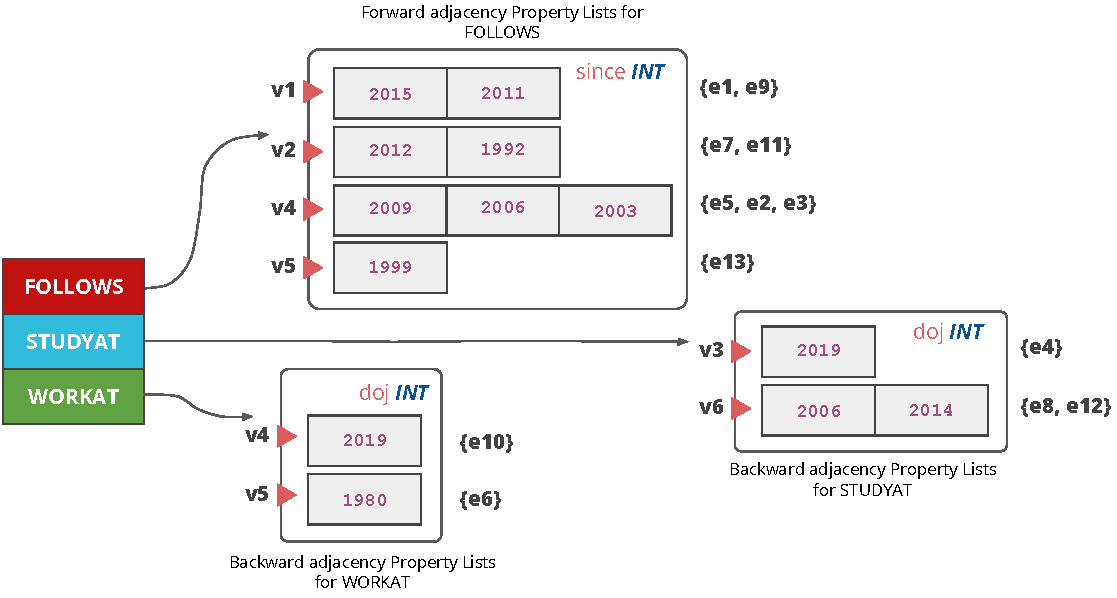
\includegraphics[scale=0.78]{img/single-dir-prop-list}\hspace*{\fill}
	\captionsetup{justification=centering}
	\caption{Single-directional Adjacency Property Lists}
	\label{fig:single-dir-prop-list}
	\vspace{0pt}
\end{figure}

Figure~\ref{fig:single-dir-prop-list} shows the Single-directional Adjacency Property Lists for storing the properties of the example graph in Figure~\ref{fig:runn}. There are 3 families, one for each edge label. Edge properties in the family of FOLLOW and WORKAT labels are stored in the forward adjacency property lists, while in STUDYAT the properties are in the backward adjacency property lists.

To access a property of an edge $e$ having label $le_i$, we need 3 pieces of information; 1) $q_{i,j}$; 2) source vertex if the $q_{i,j}$'s values are stored in the forward adjacency property lists, else destination vertex; and 3) the (list-level) positional offset of $e$ in that property list. For instance, in figure~\ref{fig:single-dir-prop-list}, \texttt{since} property of $e2$ can be accessed knowing $v4$ (source vertex of $e2$) and offset of $e2$ in $v4$'s forward adjacency property list, i.e 1. As was the case with global vertex ID, global edge IDs also cannot be used as the positional offset in the list to access a property. Hence, we adopt a new edge identification scheme that identifies the edge in the system by a tuple having 4 components: \textbf{\emph{(edge label, source vertex, destination vertex, list-level positional offset)}}. In our new scheme, the $e2$'s ID will be given as \texttt{FOLLOWS:v4:v1:2}, where $v4$ and $v1$ are the source and destination edges of $e2$. These edge IDs provides us with compact storage too. Most of the components need not be stored in the adjacency lists and the edge ID can be constructed during query execution by reading as less as only the neighbour vertex's local positional offset in the property list. 

\begin{figure}
	\vspace{-25pt}
	\hfill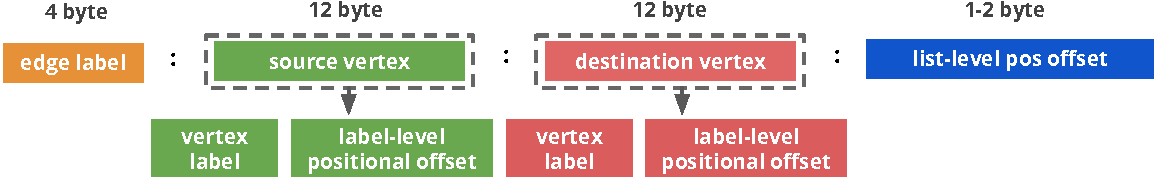
\includegraphics[scale=0.78]{img/edge-scheme}\hspace*{\fill}
	\captionsetup{justification=centering}
	\caption{Components of the new Edge identification scheme.}
	\label{fig:edge-scheme}
\end{figure}

\vspace{-12pt}
\subparagraph{Limitations.}Though single-directional adjacency property lists are as a good middle-ground solution, insertions in the list are still costly. In particular, the following are the downside of this solution:
\begin{itemize}
	\item \textbf{Costly insertions:} Insertions are costly if the edges are sorted in the adjacency lists. For example, assume a scenario where a new edge $e$ is inserted at \emph{position 5} in the forward adjacency list $A$ of vertex $v$ having a size \emph{10}. If the edge properties of $e$ are to be stored in the forward adjacency property lists of $v$, each property list will have to be rearranged. This will change the positional offset of the existing edges at location $\geq5$ in $A$. Updating the positional offsets of these edges in their occurrence in the other adjacency list requires accessing and traversing $n$ adjacency lists, which is costly.
	
	\item \textbf{Huge memory overhead:} Apart from costly insertions, a property list per edge property per vertex requires keeping a pointer to each of the lists which contributes significantly to the overall memory footprint for storing edge properties.
\end{itemize}

\vspace{-16pt}
\subparagraph{Modifications.}Clearly, insertions to the property lists are costly because edges are ordered in the adjacency lists and the property lists mimic that order too. Hence, to make insertions easy, we omit the proposition of keeping property lists ordered. By giving up ordering, queries no longer read the edges' property value sequentially while joining from the adjacency list and reading from the identically-ordered property lists. Instead, we read properties from close-by locations in a \emph{page} and still able to maintain cache locality in reads.

We store the property values of $n$ property lists in one unordered page. We call this page, a \emph{single directional adjacency property page}. The mapping from a property list to its corresponding page is straightforward. Single-directional adjacency property list for vertex $v$ and property $q_{i,j}$ maps to the $i$th page for property $q_{i,j}$, where $i$ is mod $n$ of $v$'s local positional offset. The benefit of using pages comes from it being unordered. This makes new edge insertions easy as now, the new edge properties get appended into their respective pages or recycle the location of an already deleted edge, similar to how insertions happen in vertex property columns. 

\begin{figure}
	\vspace{-40pt}
	\hfill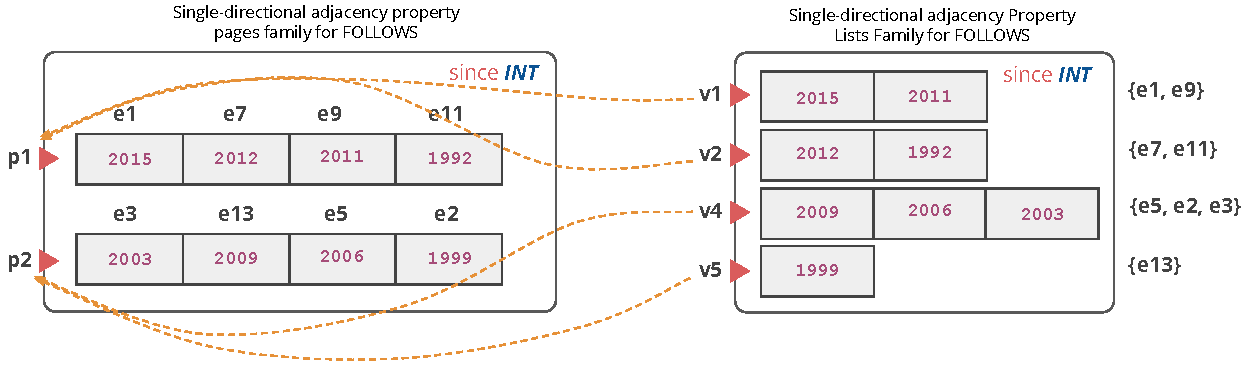
\includegraphics[scale=0.78]{img/paged}\hspace*{\fill}
	\captionsetup{justification=centering}
	\caption{Mapping single-directional adjacency property lists to single-directional adjacency property pages for since property in Figure~\ref{fig:runn}.$n=2$.}
	\label{fig:paged}
	\vspace{-5pt}
\end{figure}

Figure~\ref{fig:paged} shows the mapping of a single-directional adjacency property lists to single-direstional adjacency property pages for $n=2$. The paged edge property column has two pages that stores the property values from vertex groups $(v1,v2)$ and $(v3,v4)$ respectively, assuming that the local positional offset of $vi$ is $i$ and $pi$ is the $i$th property page for \texttt{since} property. 

The value of $n$ is chosen such that edges' property values are not too far apart from each as they were stored in the property lists. This reduces the cache miss to occur with \emph{each} access of a value in a page. Hence, the value of $n$ is dependant on 3 factors: 1) the cache line size; 2) width of an element in the page, and 3) the average number of edges in the adjacency lists. Ideally, the value of n is optimum in the range $[32, 512]$. We show in evaluation that our solution is not significantly worse than the single-directional adjacency property lists when performing sequential reads. Comparing the two, we get that our solution is 1.2x slower at the maximum for read-intensive workloads. Running the same workload using unordered edge property columns, accessing the edge properties is 4.5x slower than single-directional adjacency property lists.

\section{Columns for 1-1, 1-n, n-1 Cardinality Edges}
\label{sec:cols-for-single-cardinality}

Single cardinality labels are edge labels that have one of the following cardinalities, 1) 1..1 (one-to-one), 2) 1..n (one-to-many), and 3) n..1 (many-to-one). Such labels guarantee that there will be at most a single edge from the source vertex or to the destination vertex. For instance, let us consider an edge label BIRTHDAY that connects a vertex of type PERSON to the vertex of type DATE. Cardinality of BIRTHDAY is \emph{many-to-one}. That is, a vertex PERSON is connected to only one vertex of type DATE, while a vertex DATE can have connections to multiple PERSONs through the edge of label BIRTHDAY.

Single cardinality labels provide the opportunity of optimizing how the edges of such labels are stored. We use the fact that an edge $e$ of a single cardinality label is the \emph{only} element in either the forward adjacency list of $e$'s source vertex or forward adjacency list of $e$'s destination vertex or both. 

...


\section{Storing Edges and Vertices in Adjacency Lists}
\label{sec:storage-optimizations}

In this section, we show how vertices and edges can be stored compactly in the adjacency lists using the new identification schemes that we introduced in Sections \ref{sec:vertex-property-columns} and \ref{sec:edge-property-columns}. In particular, decomposing the ID into multiple small components enables us to either avoid storing components which are unnecessary or can be inferred, or store it in a compressed fashion using one of the compression techniques we describe in Chapter~\ref{columnar-compression}.

The new edge identification scheme recognizes an edge with 4 components: 1) edge label, 2) source vertex, 3) destination vertex and 4) local positional offset in the property pages of its properties. However, while storing the edge in an adjacency list, the edge label, source and destination vertex components can be omitted. For instance, while storing an edge $e(u,v)$ having edge label $le_i$ in the $u$'s adjacency list of $le_i$ edges, we store projection of $e$'s ID with $le_i$ and $u$ factored out. $v$ is not stored either since the neighbour vertex is stored beside each edge by default. Finally, the positional offset can be stored cheaply as often they are not more than 1 or 2 bytes hence. This follows from the fact that the number of edges in most of the adjacency list is relatively small (by the power-law) and so are the number of elements in each page. 

To sum up, each entry in the adjacency list stores a small (1-2 byte) positional offset and the neighbour vertex ID which itself comprises of vertex label and local positional offset. We now present some common scenarios that allow for even further compaction by choosing to omit to store certain components:

\begin{itemize}
	\item \textbf{When the edge label can determine the neighbour vertex label.} We know from Guideline~\ref{gdln:graph-schema} that the edge labels can determine the source or destination vertex labels whose vertices can have that label's edge. Using this information, we can determine the neighbour vertex labels in an adjacency list with edges of a single edge label. For instance, our example graph in Figure~\ref{fig:runn} contains edges having label FOLLOWS only between vertices having label PERSON. Hence, joining from any of PERSON vertex's forward (or backward) adjacency lists with edges having label FOLLOWS, we can be inferred that all the neighbour vertices in the adjacency list have label PERSON. For cases when the edge label has only a single neighbour vertex label, explicitly storing the same neighbour vertex label with each edge in the adjacency list can be avoided. This limits this optimization only to the case when the cardinality of source or destination vertex labels set of an edge label is 1. Still, the optimization holds much relevance since edge labels in the graph data are mostly defined between a single source and destination vertex label. 
	
	\item \textbf{When the edge label does not have properties.} In the absence of any properties on edges having label $le_i$, i.e, the set of structured properties determined by $le_i$ is empty, the page-level positional offset of $le_i$ edges is undefined. We can store such edges in the adjacency list without their positional offsets. With page-level positional offset undefined, an edge cannot be identified globally since there can be multiple edges with unique \emph{(edge label, source vertex, destination vertex)} tuple. We reason that there is no need for an edge to be \emph{identifiable} in the system if not for accessing its properties. Conventionally, the purpose an  \texttt{edgeID} has been two-fold, 1) to connect the source and destination vertices and, 2) to reference edge properties (if present). We can still fulfil 1) while 2) stands void in the current scenario. 
	
	\item \textbf{When the edge label has cardinality 1-1, 1-n, n-1.} As detailed in Section~\ref{sec:cols-for-single-cardinality}, we do not need positional offsets for accessing edge properties of edges having label cardinality 1-1, 1-n, n-1, which can be done directly using the positional offset of either the source or destination vertex.
	
\end{itemize}

Using the new identification scheme and further applying the above-mentioned optimizations, the adjacent edges and neighbour vertices in adjacency lists by as less as a single piece of information. We can still further reduce the memory footprint of adjacency lists by applying compression on components of the edge that has to be stored after removing unnecessary ones. We use \emph{fixed-bitwidth NULL compression}, which we describe in Section~\ref{sec:col-existing}, to compress the components of edge in the adjacency lists. Using this technique, a particular component of each edge in an adjacency list is encoded as fixed-width elements by removing a common number of leading zero bytes (that will be determimined by the maximum element) from each of them. For example, if an adjacency list has edge $[e1, e2, e3, e4, e5]$ with the neighbour vertex labels $[1, 2, 1, 1, 2]$, then the neighbour vertex label is encoded in 1 byte in the adjacency list, instead of usual 4-byte INT. Similarly, if the same set of edges have neighbour's local positional offsets $[1000, 2000, 3000, 2, 1]$, then each offset is stored in 2 bytes in the adjacency list.

We show the decrease in memory footprint of the adjacency lists, with each optimization, over the LDB SnB dataset, with more than 1 billion edges, in Chapter~\ref{c:evaluation}. Our evaluations reveal that the new scheme with opportunities to perform immense compaction and compression can reduce the size of adjacency lists by upto 94x, storing barely over 6 bytes of data per indexed edge in the system.

